% !TEX encoding = UTF-8
% !TEX TS-program = pdflatex
% !TEX root = ../tesi.tex

%**************************************************************
\chapter{\textit{Background} tecnologico} \label{background}
%**************************************************************

In questo capitolo vengono presentate le tecnologie utilizzate durante lo sviluppo di \textit{moviORDER}. La realizzazione dell'applicazione ha permesso l'apprendimento di nuove tecnologie e l'approfondimento di alcune già in parte conosciute. Alcune di queste sono state scelte dallo stagista in seguito al completamento dell'analisi dei requisiti, mentre la maggior parte sono state imposte dal \textit{tutor} aziendale o dal dominio del problema. Le tecnologie scelte dallo stagista sono state concordate con il \textit{team} di sviluppo di \visione{}. Le prossime sezioni presentano le tecnologie in base al contesto in cui sono state utilizzate.

\section{\textit{Framework}}	

La presentazione delle tecnologie utilizzate per lo sviluppo di \textit{moviORDER} comincia dalla scelta del \textit{framework}, in quanto il \textit{framework} scelto ha imposto l'utilizzo di alcuni linguaggi di programmazione usati durante il periodo di \textit{stage}. Poiché il progetto richiedeva la realizzazione di un'applicazione che funzionasse in ambiente \textit{Android} e \textit{iOS}, il \textit{tutor} aziendale ha consigliato l'utilizzo di un \textit{framework cross-platform}. Questo perché data la diversità delle tecnologie richieste per lo sviluppo di codice nativo \textit{Android} e \textit{iOS}, e la limitata quantità di tempo a disposizione per la realizzazione del progetto, l'utilizzo di un \textit{framework cross-platform} era la migliore soluzione per portare a termine il progetto nei tempi richiesti. Allo stagista è stato richiesto di decidere tra due \glossaryItem{framework cross-platform}: \textit{Xamarin} e \textit{PhoneGap}.\\ Vengono di seguito descritti:
\begin{enumerate}
	\item le motivazioni alla base dei \textit{framework cross-platform};
	\item gli approcci alla base dei \textit{framework cross-platform};
	\item il \textit{framework Xamarin};
	\item il \textit{framework PhoneGap};
	\item le motivazioni che hanno portato \textit{PhoneGap} a prevalere su \textit{Xamarin}.
\end{enumerate}

\subsection{Motivazioni alla base dei \textit{framework cross-platform}}

Al giorno d'oggi è impensabile realizzare un'applicazione \textit{mobile} per una sola piattaforma perché il mercato è eccessivamente frammentato. Quindi, se si dovesse scegliere di sviluppare un'applicazione per una sola piattaforma si perderebbe una potenziale parte di clienti. La seguente figura mostra, a scopi illustrativi, la frammentazione del mercato italiano nel 2016.

\begin{figure}[!h] 
    \centering 
    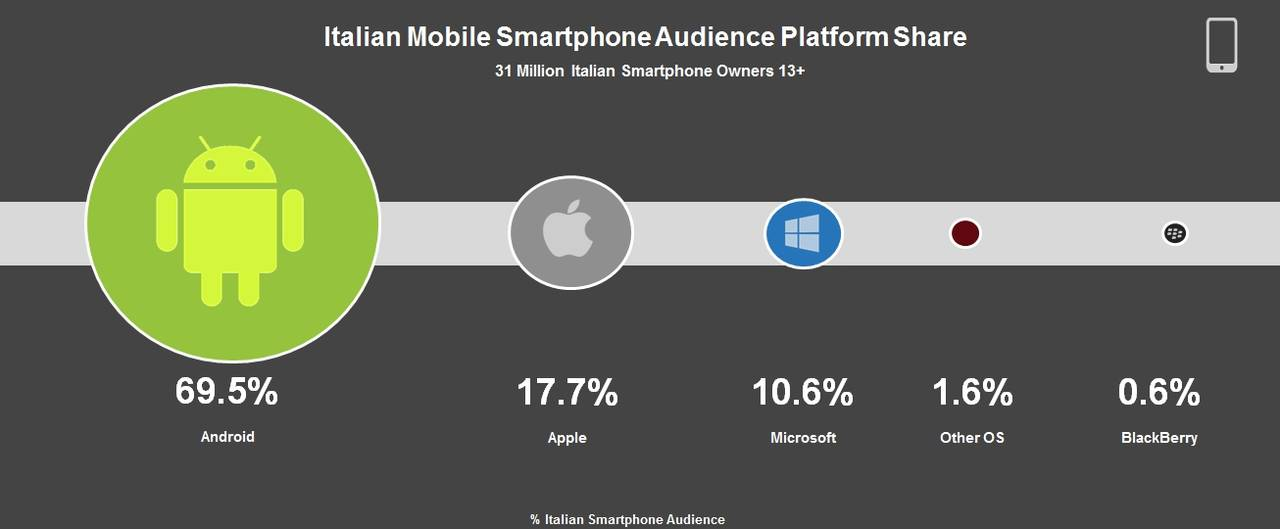
\includegraphics[width=\columnwidth]{tecnologie/mercato} 
    \caption{Frammentazione dei sistemi operativi nel mercato italiano del 2016}
\end{figure}

Compresa la necessità di sviluppare più versioni della medesima applicazione in diverse piattaforme, il problema si sposta sulle risorse economiche e sul tempo che si ha a disposizione per lo sviluppo. Infatti sviluppare in diverse piattaforme comporta l'utilizzo di differenti linguaggi di programmazione e quindi la necessità di avere più programmatori esperti, precisamente almeno uno per piattaforma. Altre variabili di cui tener conto sono gli strumenti di sviluppo necessari, le \glossaryItem{API} che si hanno a disposizione e fattori quali i sensori disponibili sui dispositivi, la dimensione degli schermi e le capacità di calcolo differenti.

L'obiettivo dei \textit{framework cross-platform} è la risoluzione di tutti questi problemi in maniera efficiente ed efficace in termini di risorse utilizzate, quindi, più precisamente, la riduzione degli effetti negativi della frammentazione del mercato.

\begin{figure}[!h] 
    \centering 
    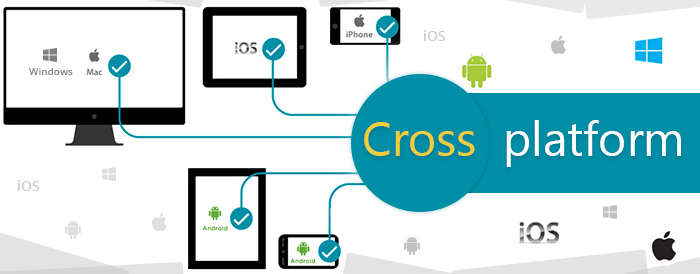
\includegraphics[width=\columnwidth]{tecnologie/framework} 
    \caption{Significato di \textit{cross-platform}}
\end{figure}

Per raggiungere questo obiettivo i \textit{framework cross-platform} consentono di utilizzare un solo linguaggio di programmazione, o un insieme ristretto di linguaggi, per sviluppare un unico codice sorgente, che viene poi convertito nel codice nativo delle piattaforme sulle quali si desidera distribuire l'applicazione. 

Per concludere, dati oggettivi dimostrano che durante il 2016 l'utilizzo dei \textit{framework cross-platform} ha permesso un risparmio in termini di risorse economiche nell'80\% dei casi ed un risparmio di tempo nell'83\% dei casi.

\subsection{Approcci alla base dei \textit{framework cross-platform}}

Per la scelta del \textit{framework} più idoneo è stato richiesto di studiare gli approcci secondo i quali i \textit{framework} permettono la distribuzione su varie piattaforme. Esistono principalmente quattro approcci in base ai quali è possibile classificare i \textit{framework}:
\begin{itemize}
	\item approccio \textit{web};
	\item approccio ibrido;
	\item approccio interpretato;
	\item approccio \glossaryItem{cross-compiled}.
\end{itemize}

In questa tesi vengono presentati solamente l'approccio ibrido e quello interpretato, poiché utilizzati dai \textit{framework} proposti dal \textit{tutor} aziendale.

L'approccio ibrido si interpone tra la realizzazione di un'applicazione \textit{web} e lo sviluppo di un'applicazione \textit{mobile} in codice nativo. In questo tipo di approccio l'applicazione viene sviluppata utilizzando tecnologie \textit{web} ed eseguita all'interno di un \glossaryItem{container} nativo sul dispositivo \textit{mobile}. Per eseguire l'applicazione viene utilizzato il motore di \textit{rendering} del \textit{browser} del dispositivo, il quale si occupa di interpretare e visualizzare il contenuto \glossaryItem{HTML} (\textit{HyperText Markup Language}) dell'applicazione tramite una visualizzazione \textit{web} a schermo intero. L'accesso alle funzionalità native offerte dal dispositivo è permesso grazie ad un livello astratto che si interpone tra l'applicazione ibrida e tali funzionalità. Questo livello astratto espone le funzionalità tramite \textit{API} \textit{Javascript}. 

\begin{figure}[!h] 
    \centering 
    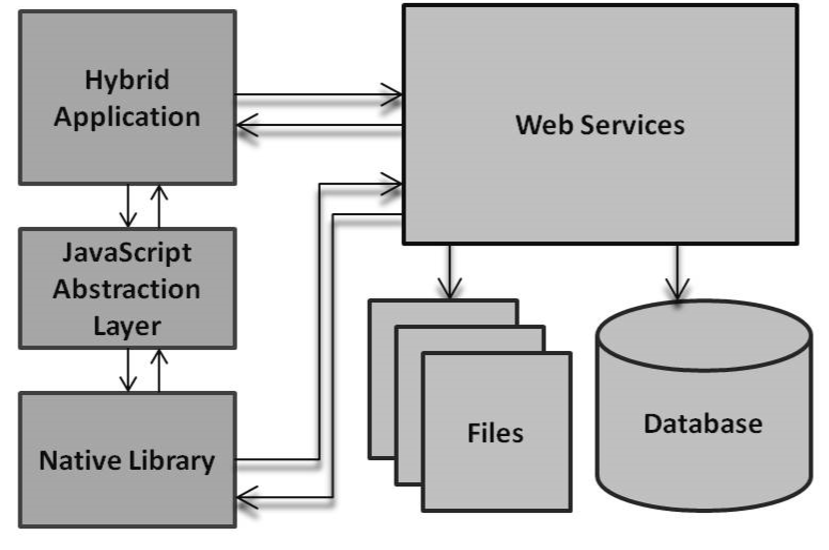
\includegraphics[width=0.9\columnwidth]{tecnologie/ibrido} 
    \caption{Architettura di un'applicazione ibrida}
\end{figure}

\newpage

Nel caso delle applicazioni interpretate il codice sorgente dell'applicazione viene distribuito sul dispositivo \textit{mobile}, dove viene successivamente interpretato da un \glossaryItem{interprete} che si occupa di eseguire il codice a \glossaryItem{run-time}. Lo sviluppo \textit{cross-platform}  è supportato dall'interprete, che permette di eseguire il codice sorgente du differenti piattaforme. L'applicazione interpretata interagisce con un livello astratto per accedere alle \textit{API} native. Un vantaggio di questo approccio è che utilizza elementi delle specifiche interfacce grafiche native per l'interazione utente. Infine, la logica applicativa viene prelevata in maniera del tutto indipendente dalla piattaforma sulla quale l'applicazione viene eseguita.

\begin{figure}[!h] 
    \centering 
    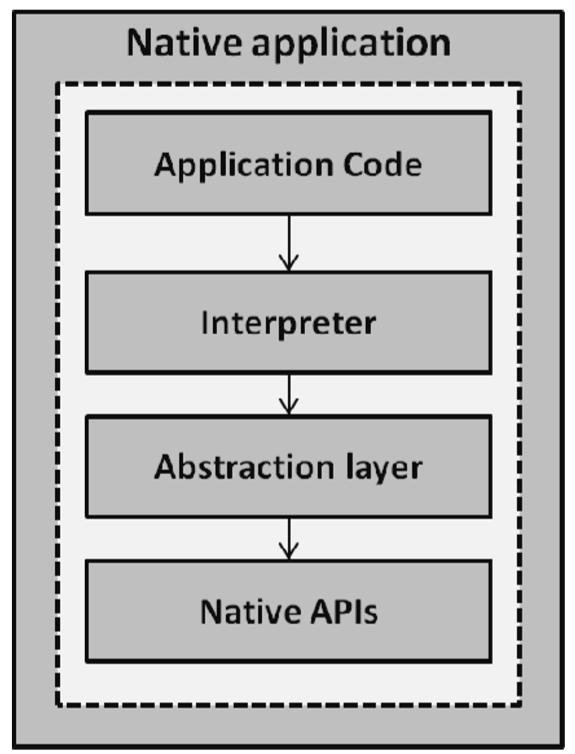
\includegraphics[height=8cm,width=0.6\columnwidth]{tecnologie/interpretato} 
    \caption{Architettura di un'applicazione interpretata}
\end{figure}

\newpage

\subsection{\textit{Xamarin}}

\textit{Xamarin} è un \textit{framework cross-platform} di proprietà dell'azienda \textit{Microsoft}, il quale utilizza due approcci differenti: l'approccio interpretato per l'ambiente \textit{Android} e \textit{Windows}, e l'approccio \textit{cross-compiled} per l'ambiente \textit{iOS}. Più precisamente, per le piattaforme \textit{Android} e \textit{Windows} è possibile generare l'applicazione direttamente tramite i \textit{tool} messi a disposizione dal \textit{framework} e successivamente distribuirla sui rispettivi \textit{store}, mentre per la piattaforma \textit{iOS} è necessario un passo aggiuntivo. Infatti, per eseguire la compilazione dell'applicazione è richiesto il passaggio per una macchina \textit{Apple} che abbia installato \textit{XCode}. Infine, \textit{Xamarin} richiede che per lo sviluppo dell'applicazione venga utilizzato il linguaggio \glossaryItem{C\#}. Nella figura sottostante viene presentata l'architettura di \textit{Xamarin}.

\begin{figure}[!h] 
    \centering 
    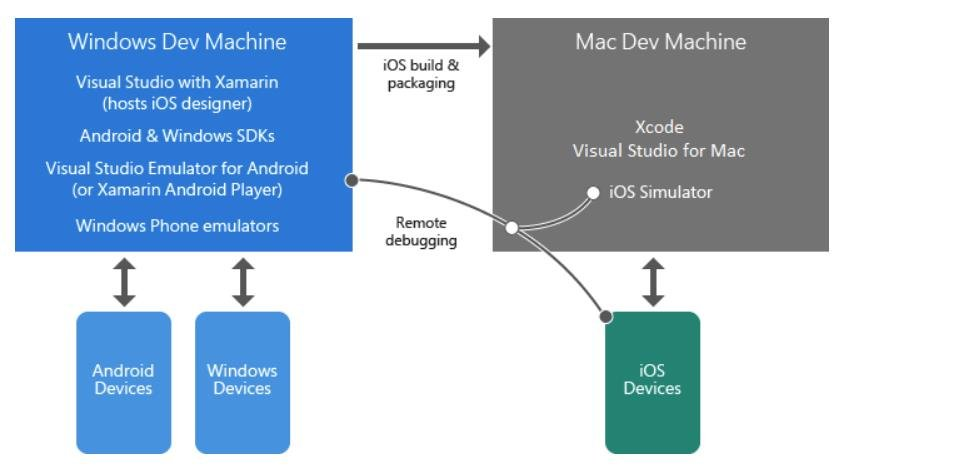
\includegraphics[width=\columnwidth]{tecnologie/xamarinArchitecture} 
    \caption{Architettura del \textit{framework Xamarin}}
\end{figure}

\subsection{\textit{PhoneGap}}

\textit{PhoneGap} è un \textit{framework cross-platform} di proprietà dell'azienda \textit{Apache}, il quale utilizza un approccio ibrido. Quindi permette la realizzazione di applicazioni \textit{mobile} tramite l'utilizzo di tecnologie \textit{web}, che sono al giorno d'oggi strumenti conosciuti da tutti gli sviluppatori. L'accesso ai componenti \textit{hardware} dei dispositivi \textit{mobile} è permesso grazie all'utilizzo di \textit{plugin} scaricabili dalla pagina ufficiale del \textit{framework}. Vantaggi importanti del \textit{framework} sono la presenza di documentazione completa per i \textit{plugin} e l'esistenza di una \glossaryItem{community} grande e disponibile. Infine, \textit{PhoneGap} rende disponibili degli strumenti che facilitano lo sviluppo dell'applicazione: \textit{PhoneGap Desktop App}, \textit{PhoneGap CLI}, \textit{PhoneGap App} e \textit{PhoneGap Build}. I primi tre verranno descritti successivamente, in quanto fanno parte dell'ambiente di sviluppo utilizzato durante lo \textit{stage}. \textit{PhoneGap Build} è uno strumento che permette di eseguire la \textit{build} dell'applicazione direttamente su un \textit{server} \textit{cloud Adobe}, a partire da un \textit{file zip} contenente la cartella con il codice sorgente dell'applicazione. In seguito alla \textit{build} è possibile generare e scaricare automaticamente l'applicazione per \textit{Windows} o \textit{Android}. Per \textit{iOS} è necessario fornire i certificati richiesti da \textit{Apple} per la distribuzione dell'applicazione. Nella pagina successiva vengono presentate l'architettura di \textit{PhoneGap} e una figura illustrativa di \textit{PhoneGap Build}.

\begin{figure}[!h] 
    \centering 
    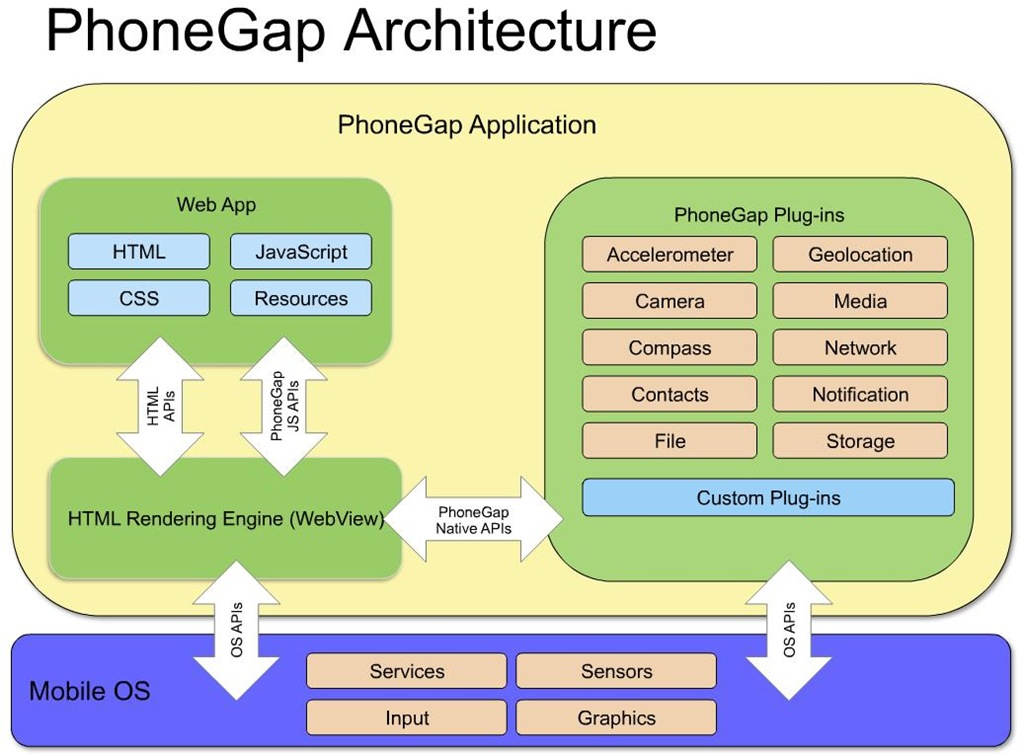
\includegraphics[width=0.9\columnwidth]{tecnologie/phonegapArchitecture} 
    \caption{Architettura del \textit{framework PhoneGap}}
\end{figure}

\begin{figure}[!h] 
    \centering 
    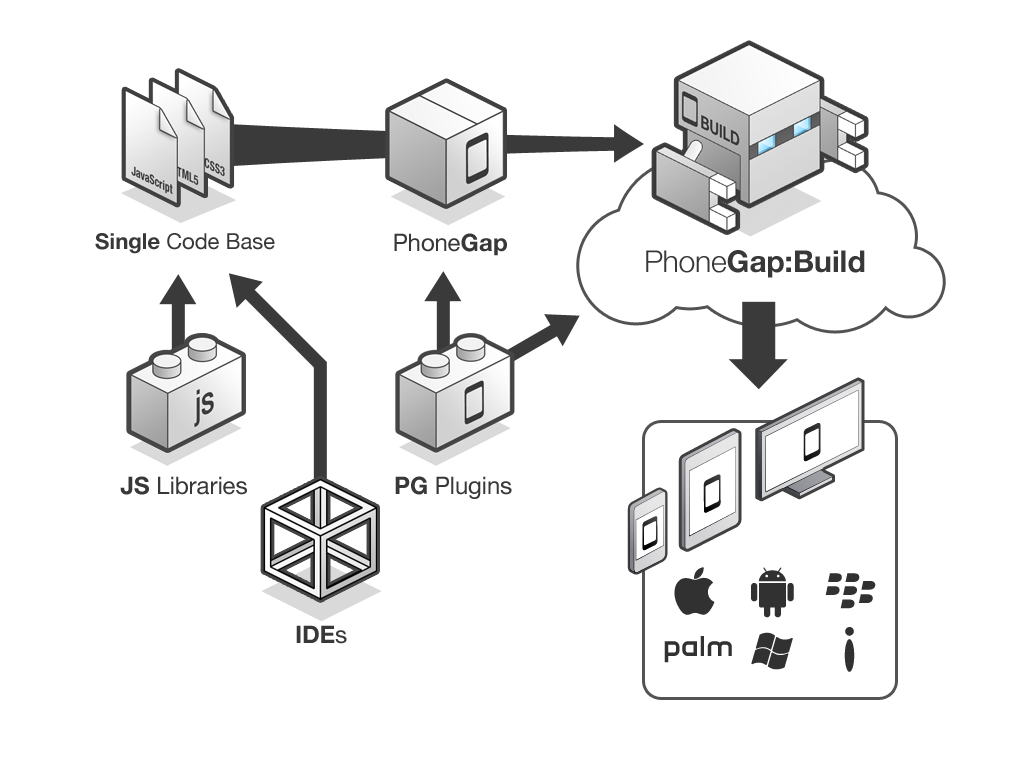
\includegraphics[width=\columnwidth]{tecnologie/phonegapBuild} 
    \caption{Figura illustrativa di \textit{PhoneGap Build}}
\end{figure}

\newpage


\subsection{La scelta di \textit{PhoneGap}}

I motivi per i quali lo stagista ha optato per il \textit{framework PhoneGap} sono i seguenti:
\begin{enumerate}
	\item \textbf{linguaggio di programmazione}: \textit{PhoneGap} richiedeva l'utilizzo di tecnologie \textit{web} già conosciute e apprese dallo stagista all'Università. Lo studio del linguaggio \textit{C\#} imposto da \textit{Xamarin} avrebbe richiesto un periodo di formazione maggiore delle 40 ore messe a disposizione per lo studio delle tecnologie;
	\item \textbf{linguaggio \textit{Javascript}}: come detto precedentemente, lo stagista era interessato ad approfondire il linguaggio \textit{Javascript}, poiché richiesto al giorno d'oggi dalla maggior parte delle aziende che si occupano della realizzazione di applicazioni \textit{web};
	\item \textbf{facilità nello sviluppo dell'interfaccia grafica}: utilizzando tecnologie \textit{web} risultava semplice progettare e sviluppare un'interfaccia grafica \glossaryItem{responsive}, in grado di adattarsi alla maggior parte dei dispositivi \textit{mobile} presenti sul mercato.
\end{enumerate}

\section{Ambiente di sviluppo}

Durante il periodo di \textit{stage} è stato utilizzato uno specifico ambiente di lavoro, comprendente tecnologie imposte dal \textit{tutor} aziendale e alcune scelte dallo stagista. La qualità delle tecnologie ha impatto diretto sulla qualità di processo e quindi su quella del prodotto, per cui è importante tenere l'ambiente di lavoro costantemente completo, ordinato e aggiornato. Per ottenere questo lo stagista ha dovuto analizzare le tecnologie scelte per assicurarsi che fossero le più adatte per il dominio del problema.

\subsection{\textit{Suite} di \textit{PhoneGap}}

La \textit{suite} di \textit{PhoneGap} ha costituito parte fondamentale dell'ambiente di lavoro. Sono stati utilizzati i seguenti \textit{software}:
\begin{itemize}
	\item \textbf{\textit{PhoneGap Desktop App}}: applicazione utilizzata inizialmente per prendere dimestichezza con il \textit{framework};
	\item \textbf{\textit{PhoneGap CLI}}: interfaccia a linea di comando utilizzata dopo aver preso dimestichezza con il \textit{framework};
	\item \textbf{\textit{PhoneGap App}}: applicazione \textit{mobile} utilizzata inizialmente per testare l'applicazione generata dal \textit{framework}.
\end{itemize}

\textit{PhoneGap Desktop App} è disponibile su \textit{Windows} o \textit{Mac} e permette di iniziare ad utilizzare il \textit{framework} con estrema facilità. Essa fornisce un'interfaccia grafica per creare, gestire e testare progetti \textit{PhoneGap}. Nella pagina successiva viene presentata una figura che mostra l'interfaccia grafica di \textit{PhoneGap Desktop App}.

\begin{figure}[!h] 
    \centering 
    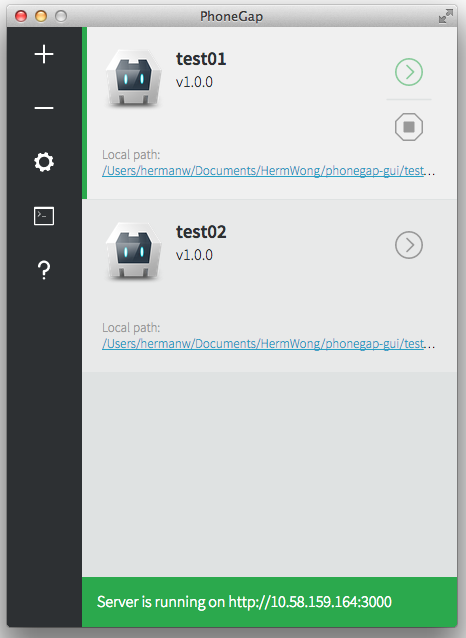
\includegraphics[width=0.8\columnwidth]{tecnologie/phonegapDesktop} 
    \caption{\textit{PhoneGap Desktop App}}
\end{figure}

\newpage

\textit{PhoneGap CLI} estende le funzionalità offerte da \textit{PhoneGap Desktop App} tramite un'interfaccia a riga di comando. Prima del rilascio dell'app desktop, \textit{PhoneGap CLI} veniva utilizzata come strumento principale per configurare e gestire il \textit{framework}. \textit{PhoneGap CLI} può essere utilizzata singolarmente oppure assieme a \textit{PhoneGap Desktop App} e/o \textit{PhoneGap Build}.

\textit{PhoneGap App} è un'applicazione \textit{mobile} che permette di testare l'applicazione \textit{PhoneGap} senza generare ed installare nessun \textit{file} applicazione. Per il test è sufficiente avviare l'esecuzione del progetto su \textit{PhoneGap Desktop App} e collegare il \textit{computer} di sviluppo con il dispositivo su cui è installata \textit{PhoneGap App}. Dopo il collegamento sarà possibile testare completamente l'applicazione.

\begin{figure}[!h] 
    \centering 
    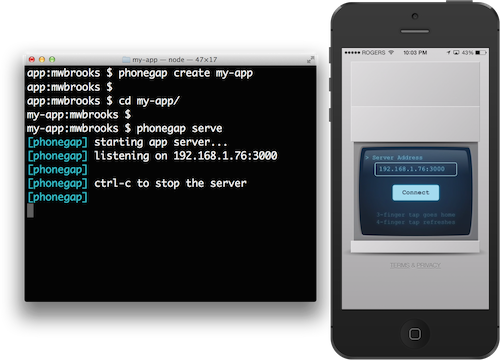
\includegraphics[width=0.8\columnwidth]{tecnologie/phonegapCLIApp} 
    \caption{\textit{PhoneGap CLI} e \textit{PhoneGap App}}
\end{figure}

\subsection{\textit{Editor} e \textit{IDE}}

\subsubsection{\textit{Sublime Text 3.0}}

Per lo sviluppo del progetto \textit{PhoneGap} è stato utilizzato l'\textit{editor} \textit{Sublime Text 3.0}, ritenuto dallo stagista il più semplice e leggero per la realizzazione di applicazioni \textit{web}. 

\begin{figure}[!h] 
    \centering 
    
\includegraphics[height=4cm,width=4cm]{tecnologie/sublime} 
    \caption{Logo di \textit{Sublime Text 3.0}}
\end{figure}

\subsubsection{\textit{Android Studio}}

Durante lo \textit{stage} l'applicazione \textit{Android} generata tramite i \textit{tool} offerti dal \textit{framework PhoneGap} non era soddisfacente: spesso non funzionava o l'interfaccia grafica non rispecchiava quella desiderata. Per rendere l'\textit{app} usabile è stato necessario installare \textit{Android Studio}, il quale ha permesso di mettere mano sul codice nativo. \textit{Android Studio} è un ambiente di sviluppo integrato (\glossaryItem{IDE}) basato sul \textit{software} di \textit{JetBrains IntelliJ IDEA} e progettato specificamente per lo sviluppo di applicazioni \textit{Android}.

\begin{figure}[!h] 
    \centering 
    
\includegraphics[height=4.5cm,width=4.5cm]{tecnologie/androidStudio} 
    \caption{Logo di \textit{Android Studio}}
\end{figure}

\subsubsection{\textit{XCode}}

Durante lo \textit{stage} l'applicazione \textit{iOS} generata tramite i \textit{tool} offerti dal \textit{framework PhoneGap} non era soddisfacente: spesso non funzionava o l'interfaccia grafica non rispecchiava quella desiderata. Per rendere l'\textit{app} usabile è stato necessario installare \textit{XCode}, il quale ha permesso di mettere mano sul codice nativo. \textit{Xcode} è un ambiente di sviluppo integrato (\textit{IDE}), sviluppato e mantenuto da \textit{Apple}, che contiene una suite di strumenti utili allo sviluppo di \textit{software} per i sistemi \textit{macOS}, \textit{iOS}, \textit{watchOS} e \textit{tvOS}.

\begin{figure}[!h] 
    \centering 
    
\includegraphics[height=4cm,width=5cm]{tecnologie/xCode} 
    \caption{Logo di \textit{XCode}}
\end{figure}

\subsubsection{\textit{Eclipse JEE}}

Durante lo \textit{stage} è stata richiesta la realizzazione di un servizio \textit{web} che si interponesse tra la logica applicativa di \textit{moviORDER} e un \textit{database} presente sul \textit{server Azure} di \visione{}. Il servizio \textit{web} è stato realizzato in linguaggio \textit{Java} tramite l'utilizzo di oggetti \textit{servlet}. Per lo sviluppo degli oggetti \textit{servlet} è stato utilizzato l'\textit{IDE Eclipse JEE}, il quale offre buoni strumenti per lo sviluppo di applicazioni \textit{web} \textit{Java}. \textit{Eclipse} è un ambiente di sviluppo integrato multi-linguaggio e multipiattaforma, ideato da un consorzio di grandi società quali \textit{Ericsson}, \textit{HP}, \textit{IBM}, \textit{Intel}, \textit{MontaVista Software}, \textit{QNX}, \textit{SAP} e \textit{Serena Software}, chiamato \textit{Eclipse Foundation}.

\begin{figure}[!h] 
    \centering 
    
\includegraphics[width=0.8\columnwidth]{tecnologie/eclipse} 
    \caption{Logo di \textit{Eclipse}}
\end{figure}

\newpage

\subsection{Gestione \textit{DBMS}}

Durante il progetto è stato utilizzato il \glossaryItem{DBMS} \textit{Microsoft SQL Server} per gestire il \textit{database} di \textit{moviORDER}. Per una gestione veloce ed ottimale dello stesso si è deciso di usare il \textit{software} \textit{SQL Server Management Studio}. \textit{SQL Server Management Studio} (\textit{SSMS}) è un'applicazione \textit{software} usata per configurare, gestire e amministrare \textit{database}, in locale o su un \textit{server cloud}, con il \textit{DBMS Microsoft SQL Server}. 

\begin{figure}[!h] 
    \centering 
    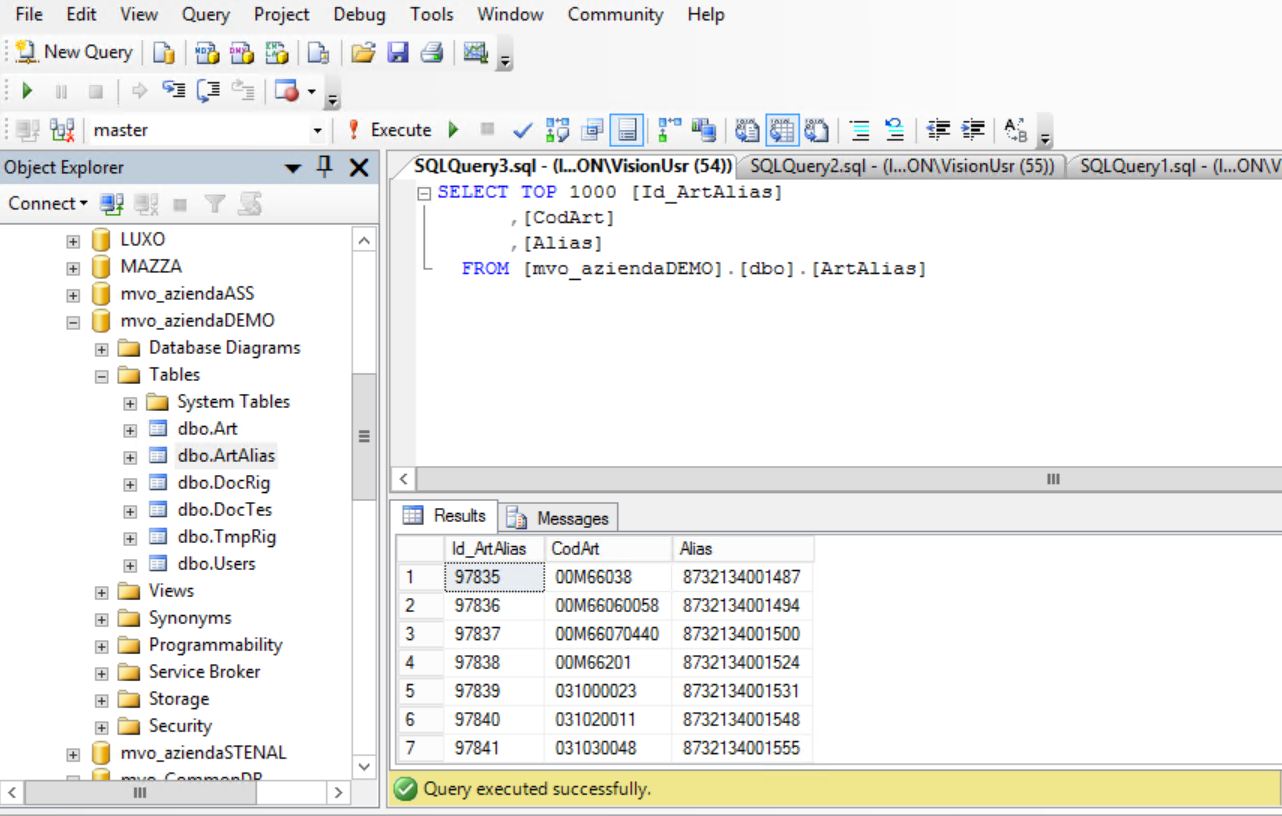
\includegraphics[width=\columnwidth]{tecnologie/ssms} 
    \caption{\textit{Screenshot} di \textit{SQL Server Management Studio}}
\end{figure}

\newpage

\subsection{\textit{Server web}}

Per permettere l'esecuzione del servizio \textit{web} sul \textit{server cloud} di \visione{} si è utilizzato \textit{Apache Tomcat}. \textit{Apache Tomcat} (o semplicemente \textit{Tomcat}) è un \glossaryItem{server web} (nella forma di contenitore \textit{servlet}) \textit{open source} sviluppato dalla \textit{Apache Software Foundation}. Implementa le specifiche \glossaryItem{JavaServer Pages} (\textit{JSP}) e \textit{servlet}, fornendo quindi una piattaforma \textit{software} per l'esecuzione di applicazioni \textit{web} sviluppate in linguaggio \textit{Java}.

\begin{figure}[!h] 
    \centering 
    
\includegraphics[height=4cm,width=5cm]{tecnologie/tomcat} 
    \caption{Logo di \textit{Apache Tomcat}}
\end{figure}

\subsection{\textit{Cloud computing}}

Il servizio \textit{web} e il \textit{database} con il quale l'applicazione interagisce risiedono su un \textit{server Azure} di \visione{}. \textit{Microsoft Azure} (precedentemente nota come \textit{Windows Azure}) è la piattaforma \textit{cloud} pubblica di \textit{Microsoft}, che offre servizi di \glossaryItem{cloud computing}. Tramite Azure vengono erogati servizi appartenenti a diverse categorie, quali: risorse di elaborazione, archiviazione e memorizzazione dati, trasmissione dati e interconnessione di reti, analisi, \textit{intelligence}, apprendimento automatico, sicurezza e gestione delle identità, monitoraggio e gestione, nonché servizi per lo sviluppo di applicazioni. Per accedere al \textit{server} da remoto è stato utilizzato il \textit{software} ``Connessione \textit{Desktop} Remoto di \textit{Windows}''.

\begin{figure}[!h] 
    \centering 
    
\includegraphics[width=0.8\columnwidth]{tecnologie/azure} 
    \caption{Logo di \textit{Microsoft Azure}}
\end{figure}

\newpage

\subsection{Strumenti di \textit{testing}}\label{postman}

Durante lo sviluppo di \textit{moviORDER} sono stati eseguiti dei test per verificare il corretto funzionamento del servizio \textit{web} e dell'applicazione. Per il test dell'\textit{API} del servizio \textit{web} si è utilizzato \textit{Postman}. \textit{Postman} è uno strumento di \glossaryItem{API testing} che permette di testare \textit{API} direttamente, o come parte di test d'integrazione, per determinare se soddisfano criteri di funzionalità, affidabilità, performance e sicurezza. Nel caso di \textit{moviORDER}, il test avviene tramite l'invio di una richiesta \textit{HTTP POST} all'\textit{API} sul \textit{server cloud}. Successivamente il \textit{software} visualizza la stringa in formato \textit{JSON} restituita dal \textit{server} e lo sviluppatore può verificare se la risposta del servizio è quella attesa.

\begin{figure}[!h] 
    \centering 
    
\includegraphics[height=4cm,width=5cm]{tecnologie/postman} 
    \caption{Logo di \textit{Postman}}
\end{figure}

Per testare il corretto funzionamento dell'applicazione si è utilizzata la \textit{console} del \textit{browser Google Chrome}, facente parte degli strumenti offerti dallo stesso per gli sviluppatori \textit{web}. Tramite la \textit{console} è stato possibile verificare il codice \textit{JavaScript} che costituisce la logica applicativa di \textit{moviORDER}.

\begin{figure}[!h] 
    \centering 
    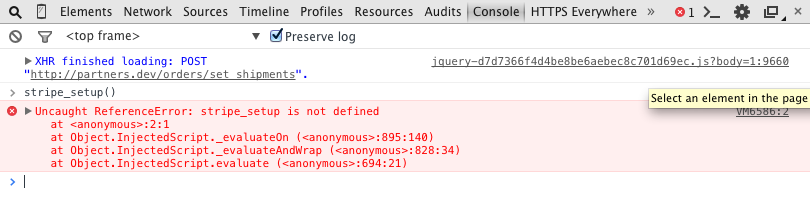
\includegraphics[width=\columnwidth]{tecnologie/console} 
    \caption{\textit{Screenshot} della \textit{console} di \textit{Google Chrome}}
\end{figure}

\newpage

\subsection{Strumenti di \textit{versioning} e \textit{ticketing}}

Per scelta dello stagista il progetto è stato sottoposto a controllo di versione in ogni sua parte: applicazione, servizio \textit{web} e documentazione. Questo ha permesso, principalmente nel caso dell'applicazione, di tornare a \glossaryItem{baseline} sicure nel caso di sovrascritture, perdite accidentali e \glossaryItem{commit} di codice con errori di programmazione. Per il controllo di versione si è utilizzato lo strumento \textit{Git} e in particolare il servizio di hosting \textit{GitHub}. Lo stagista ha scelto tali \textit{software} poiché già utilizzati in progetti didattici durante l'Università.

\begin{figure}[!h] 
    \centering 
    
\includegraphics[height=5cm,width=5cm]{tecnologie/git} 
    \caption{Logo di \textit{GitHub}}
\end{figure}

Lo stagista ha scelto inoltre di utilizzare lo strumento di \glossaryItem{ticketing} \textit{Asana}, in modo da facilitare la pianificazione del progetto. \textit{Asana} è un'applicazione \textit{web} e \textit{mobile} progettata per aiutare i \textit{team} ad organizzare, tracciare e gestire il loro lavoro. In particolare, lo strumento è stato utilizzato per dare una scadenza ai \textit{task} assegnati dal \textit{tutor} aziendale.

\begin{figure}[!h] 
    \centering 
    
\includegraphics[height=5cm,width=7cm]{tecnologie/asana} 
    \caption{Logo di \textit{Asana}}
\end{figure}

\subsection{Strumenti di modellazione e documentazione}

Il progetto ha richiesto lo sviluppo di diagrammi di \textit{Gantt} in fase di pianificazione e di diagrammi \glossaryItem{UML} (\textit{Unified Modeling Language}) in fase di analisi dei requisiti e progettazione. Per la realizzazione dei diagrammi di \textit{Gantt} si è utilizzato \textit{Gantt Project}, per i diagrammi \textit{UML} dei casi d'uso si è utilizzato \textit{Astah UML}, mentre per i diagrammi \textit{UML} dei \textit{package} e delle classi si è utilizzato \textit{Visual Paradigm CE}. I \textit{software} sono stati scelti perché già appresi durante il progetto di Ingegneria del \textit{Software} all'Università.

\begin{figure}[!h] 
    \centering 
    	\subfloat{
\includegraphics[width=0.33\columnwidth]{tecnologie/gantt}}
    	\subfloat{
\includegraphics[width=0.33\columnwidth]{tecnologie/astah}} 
    	\subfloat{
\includegraphics[width=0.33\columnwidth]{tecnologie/vp}} 
    \caption{Loghi di \textit{Gantt Project}, \textit{Astah UML} e \textit{Visual Paradigm CE}}
\end{figure}

Per la realizzazione dei diagrammi \glossaryItem{ER} (\textit{Entity Relationship}) e delle figure illustrative dell'architettura del prodotto si è utilizzato il \textit{software} \textit{Lucidchart}. Per la stesura della documentazione si è utilizzato l'\textit{editor} \textit{TexMaker}, anch'esso appreso durante il progetto di Ingegneria del \textit{Software}. \textit{TexMaker} permette l'integrazione con un dizionario per il controllo ortografico e la compilazione e visione del \textit{pdf} prodotto.

\begin{figure}[!h] 
    \centering 
    \subfloat{
\includegraphics[height=4.5cm,width=4.5cm]{tecnologie/lucid}}
    \subfloat{
\includegraphics[height=4.5cm,width=4.5cm]{tecnologie/tex}}
    \caption{Loghi di \textit{Lucidchart} e \textit{TexMaker}}
\end{figure}

\subsection{Linguaggi di programmazione e \textit{murkup}}

\subsubsection{\textit{HTML5}, \textit{CSS3} e \textit{JavaScript}}

Siccome è stato scelto il \textit{framework PhoneGap}, lo stagista ha dovuto utilizzare i linguaggi \textit{HTML5}, \glossaryItem{CSS3} e \textit{JavaScript}, in quanto \textit{PhoneGap} richiede di sviluppare l'applicazione tramite l'utilizzo di tecnologie \textit{web}. In particolare, \textit{HTML5} è stato scelto perché include un insieme di funzionalità che permettono di valorizzare le interfacce \textit{mobile}. Alcune di queste evidenziano come \textit{HTML5} sia già per sua natura orientato al \textit{mobile}. In particolare \textit{HTML5} fornisce \textit{API} per:
\begin{itemize}
	\item \textbf{geolocalizzazione}: con la scrittura di poco codice, forniscono la posizione del dispositivo in coordinate terrestri. Quindi, la stessa funzionalità su uno \textit{smartphone} o un \textit{tablet} fornisce la posizione dell'utente stesso;
	\item \textbf{eventi \textit{touch}}: mentre i meccanismi di input nei PC consistono per lo più nella tastiera e nel mouse, nei dispositivi mobili quasi tutto passa per il \textit{touch screen}, e avere funzionalità comode per gestire questo strumento consente un'interazione più ricca e senza limitazioni per l'utente. Le gestualità da attuare su un \textit{display}, nel mondo \textit{mobile}, costituiscono un vero e proprio linguaggio fondamentale nella \textit{user experience};
	\item \textbf{controllo batteria}: considerata l'importanza rivestita dalle risorse energetiche, l'esistenza stessa di questa libreria nel linguaggio dimostra come il suo impiego sia particolarmente mirato al panorama \textit{mobile}.
\end{itemize}

Ciò che ha favorito la scelta di \textit{CSS3} sono state le \glossaryItem{media queries}. Esse permettono di definire regole stilistiche in base alla tipologia del mezzo di visualizzazione, delle sue dimensioni e della sua attuale disposizione (\textit{portrait} o \textit{landscape}). Ciò influisce non solo sull'aspetto esteriore degli elementi ma anche sul loro posizionamento e quindi sulla struttura stessa dell'interfaccia.

Per quanto riguarda il linguaggio \textit{JavaScript} si è utilizzato \textit{JavaScript} puro, senza l'utilizzo di \textit{framework} o \glossaryItem{JQuery}. Una particolarità del linguaggio, detta \textit{AJAX}, ha reso possibile eseguire chiamate all'\textit{API} del servizio \textit{web} di \textit{moviORDER}. \textit{AJAX}, acronimo di \textit{\textit{Asynchronous JavaScript and XML}}, è una tecnica di sviluppo \textit{software} per la realizzazione di applicazioni \textit{web} interattive (\textit{Rich Internet Application}). Lo sviluppo di applicazioni \textit{HTML} con \textit{AJAX} si basa su uno scambio di dati in \textit{background} fra \textit{web browser} e \textit{server}, che consente l'aggiornamento dinamico di una pagina \textit{web} senza esplicito ricaricamento da parte dell'utente.

\begin{figure}[!h] 
    \centering 
    	
\includegraphics[width=0.8\columnwidth]{tecnologie/html5}
    \caption{Loghi di \textit{HTML5}, \textit{CSS3} e \textit{JavaScript}}
\end{figure}

I linguaggi scelti, grazie alle loro caratteristiche che li rendono orientati allo sviluppo \textit{mobile}, insieme ai meccanismi che il \textit{framework PhoneGap} utilizza per convertire una \textit{web application} in un'applicazione \textit{mobile}, permettono di effettuare meno modifiche in seguito per perfezionare l'applicazione su \textit{Android} e \textit{iOS}.

\subsubsection{\textit{Java}}

Per la realizzazione del servizio \textit{web} si è utilizzato il linguaggio \textit{Java}. La scelta poteva ricadere su \textit{Java} o \glossaryItem{PHP} (\textit{HyperText Preprocessor}). È stato scelto \textit{Java} in quanto possiede un compilatore, risulta più facilmente ``\textit{debuggabile}'' rispetto a \textit{PHP} e permette l'utilizzo di oggetti \textit{servlet}. I \textit{servlet} sono oggetti \textit{Java} che operano all'interno di un \textit{server web}, oppure un \textit{server} per applicazioni, che permettono la creazione di un'applicazione \textit{web}. Nel caso del progetto, i \textit{servlet} hanno permesso lo sviluppo dell'\textit{API} che costituisce il servizio \textit{web}. Una descrizione dell'\textit{API}, di come i \textit{servlet} sono stati utilizzati nel progetto e di come l'\textit{API} viene interrogata dall'applicazione, è presente in sezione §\ref{api}.

\begin{figure}[!h] 
    \centering 
    
\includegraphics[height=4.5cm,width=4.5cm]{tecnologie/java} 
    \caption{Logo di \textit{Java}}
\end{figure}

\subsubsection{\LaTeX{}}

Per la stesura della documentazione annessa a \textit{moviORDER} è stato utilizzato il linguaggio \LaTeX{}. La scelta è ricaduta su \LaTeX{} poiché già appreso e utilizzato durante il progetto di Ingegneria del \textit{Software}. \LaTeX{} è un linguaggio di \textit{markup} usato per la preparazione di testi, basato sul programma di composizione tipografica \TeX{}. Fornisce funzioni di \glossaryItem{desktop publishing} programmabili e mezzi per l'automazione della composizione tipografica, inclusa la numerazione, i riferimenti incrociati, tabelle e figure, organizzazione delle pagine, bibliografie e molto altro. Infine la particolarità più utile del linguaggio è l'esistenza di \textit{community} che rendono disponibili \glossaryItem{template} riutilizzabili, come quello che è stato utilizzato per la stesura di questa tesi.

\begin{figure}[!h] 
    \centering 
    
\includegraphics[height=3cm,width=6cm]{tecnologie/latex} 
    \caption{Logo di \LaTeX{}}
\end{figure}

\subsection{\textit{DBMS}}

Per la creazione, gestione e amministrazione di \textit{database} è stato utilizzato il \textit{DBMS Microsoft SQL Server}. È stato scelto questo \textit{software} poiché già ampiamente utilizzato all'interno di \visione{}. In questo modo gli sviluppatori dell'azienda potranno occuparsi della manutenzione del \textit{database} di \textit{moviORDER} con un \textit{DBMS} conosciuto. \textit{Microsoft SQL Server} usa una variante del linguaggio \glossaryItem{SQL} (\textit{Structured Query Language}) standard chiamata \glossaryItem{Transact-SQL} (\textit{T-SQL}). \textit{Transact-SQL} espande le prestazioni di \textit{SQL} aggiungendo:
\begin{itemize}
	\item funzioni per controllo di flusso;
	\item possibilità di definire variabili locali;
	\item varie funzioni per la manipolazione di stringhe, date ed espressioni matematiche;
	\item miglioramento delle istruzioni \textit{DELETE} e \textit{UPDATE}.
\end{itemize}

\begin{figure}[!h] 
    \centering 
    
\includegraphics[height=5cm,width=7cm]{tecnologie/sqlserver} 
    \caption{Logo di \textit{SQL Server}}
\end{figure}